

\section*{Declaración de Cumplimiento}


En cumplimiento de lo dispuesto en el Convenio de Chicago de 1944, el Decreto 1294 de 2021 y el Reglamento Aeronáutico Colombiano RAC 100, \textbf{Skyfilms S.A.S.}, como explotador de Sistemas de Aeronaves No Tripuladas (UAS) en la Categoría Específica, emite la presente Declaración de Cumplimiento:

\begin{enumerate}
    \item Skyfilms S.A.S. manifiesta que todas sus operaciones aéreas con UAS se desarrollan en estricto apego a las disposiciones establecidas en el RAC 100 y demás normas aeronáuticas vigentes en la República de Colombia.
    \item Las operaciones de la compañía se restringen exclusivamente a la \textbf{simple captura de imágenes o datos} con fines audiovisuales y comerciales. 
    \item Se declara expresamente que todas las misiones se ejecutarán bajo la modalidad de \textbf{Visibilidad en Línea de Vista (VLOS)}, incluyendo autorizaciones para \textbf{Vuelo Nocturno}. Quedan estrictamente excluidas las operaciones más allá de la línea de vista (BVLOS), operaciones de línea de vista extendida (EVLOS) y el transporte de carga (\textit{Drone Delivery}).
    \item La empresa se compromete a implementar rigurosamente los procedimientos descritos en este Manual de Operaciones (MO), el Sistema de Gestión de Seguridad Operacional (SMS) y el Manual de Control de Mantenimiento (MCM), garantizando la gestión de riesgos, la protección de terceros en superficie y la preservación del espacio aéreo.
    \item Se reconoce la autoridad de la Unidad Administrativa Especial de Aeronáutica Civil (Aerocivil) como ente regulador, certificador y supervisor de las operaciones.
    \item Skyfilms S.A.S. se obliga a mantener actualizada la información contenida en este Manual, sometiendo a aprobación de la Aerocivil cualquier enmienda operativa sustancial.
\end{enumerate}

Todo el personal vinculado a Skyfilms S.A.S. está en la obligación ineludible de conocer, comprender y aplicar estrictamente todos los procesos y procedimientos contenidos en este manual.

\vspace{2cm}
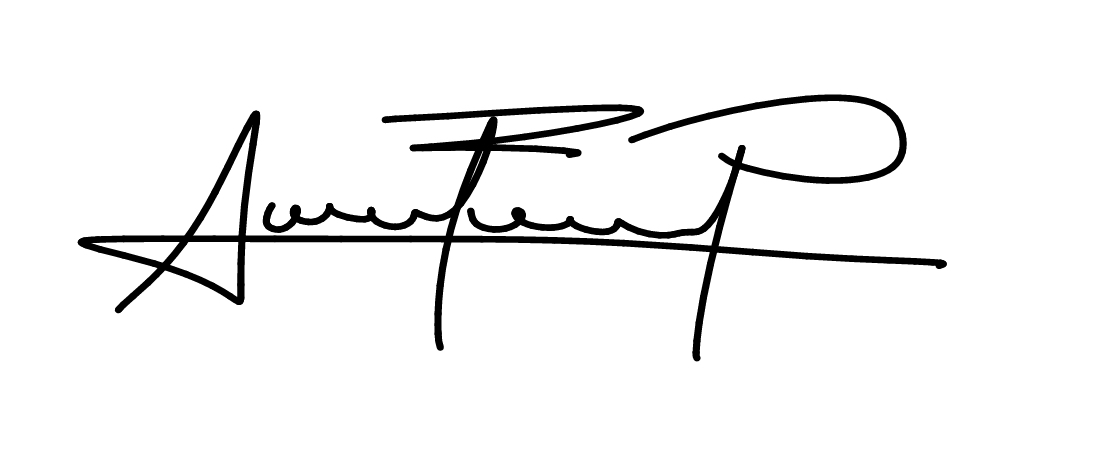
\includegraphics[width=6cm]{Imagenes/firma.jpg}

\textbf{Andrés Felipe Pérez Sierra}\\
C.C. 1.108.206.142\\
Gerente General\\
Skyfilms S.A.S.